\chapter[Gold nanorods as nano-thermometers]{Supplementary information for: Gold
nanorods as nano-thermometers}
\label{ch:SAntiStokes}

\newpage

\section{Comparing Comsol and Simple approximation for temperature calculation}
\begin{figure}[htp] \centering
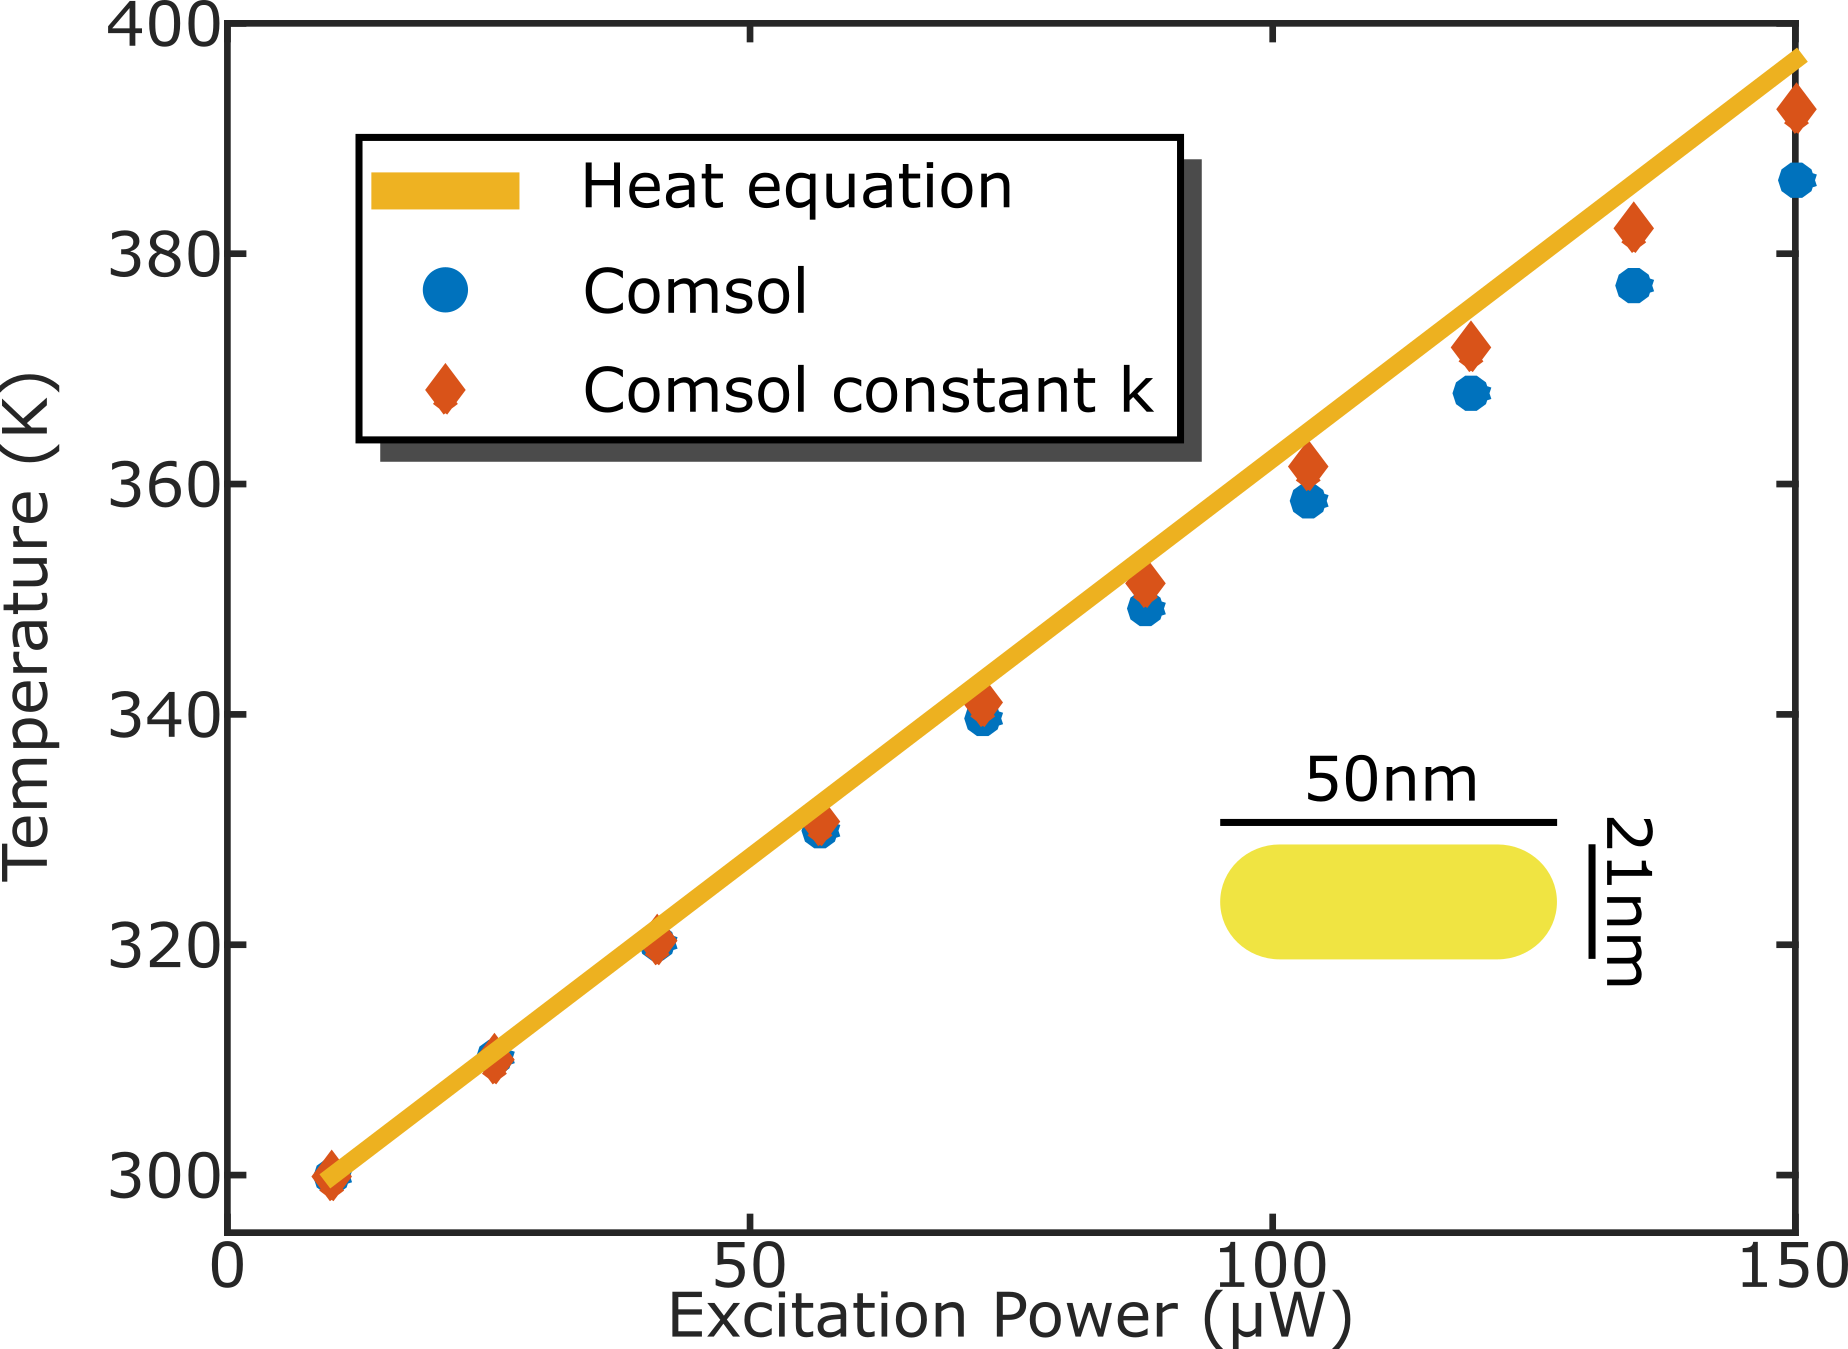
\includegraphics[width=0.5\textwidth]{Chapters/04_Anti-Stokes/Figures/Supplementary/03_Compare_Comsol/03_Compare_Comsol.png}
\caption{Calculated temperature for a $21\nm\times 50\nm$ nanorod under
different excitation intensities. The full line is the result of the simple
model while the dots are the calculated values using Comsol. The circles are
with the default heat conductivity and the diamonds are with a constant value.}
	\label{fig:Compare-Comsol}
\end{figure}

Throughout the main text the temperature measured with the anti-Stokes emission
is compared to the calculated temperature using a simple heat diffusion
equation. For spheres, assuming a thermal conductivity much higher than the
surrounding medium, the temperature increase is given by

\begin{equation}
	\Delta \textrm{T}(P) = \frac{P}{4\pi k_{\textrm{water}} R}
\end{equation}

\noindent where $P$ is the dissipated power, $k_{\textrm{water}}$ is the heat
conductivity of water and $R$ is the radius of the particle. The dissipated power can be
easily derived from the cross section of the particle at a given wavelength and
the intensity of the focused laser beam. For nanorods we assumed an
equivalent radius such that the total area is preserved.

Figure \ref{fig:Compare-Comsol} shows the difference between the results from
the equation (full line) and a finite element method calculation using Comsol
(dots) for a nanorod of length $50\nm$ and diameter $21\nm$. The cross section
and dissipated power were kept the same. The blue circles are the results given
by using the built-in material properties of water, i.e. a thermal conductivity
that depends on temperature. The diamonds are the results when the thermal
conductivity is fixed to $0.61 \W(\m\cdot\K)^{-1}$. The difference is
accentuated at higher temperatures.

\newpage

\section{Luminescence power dependence}
\begin{figure}[htp] \centering
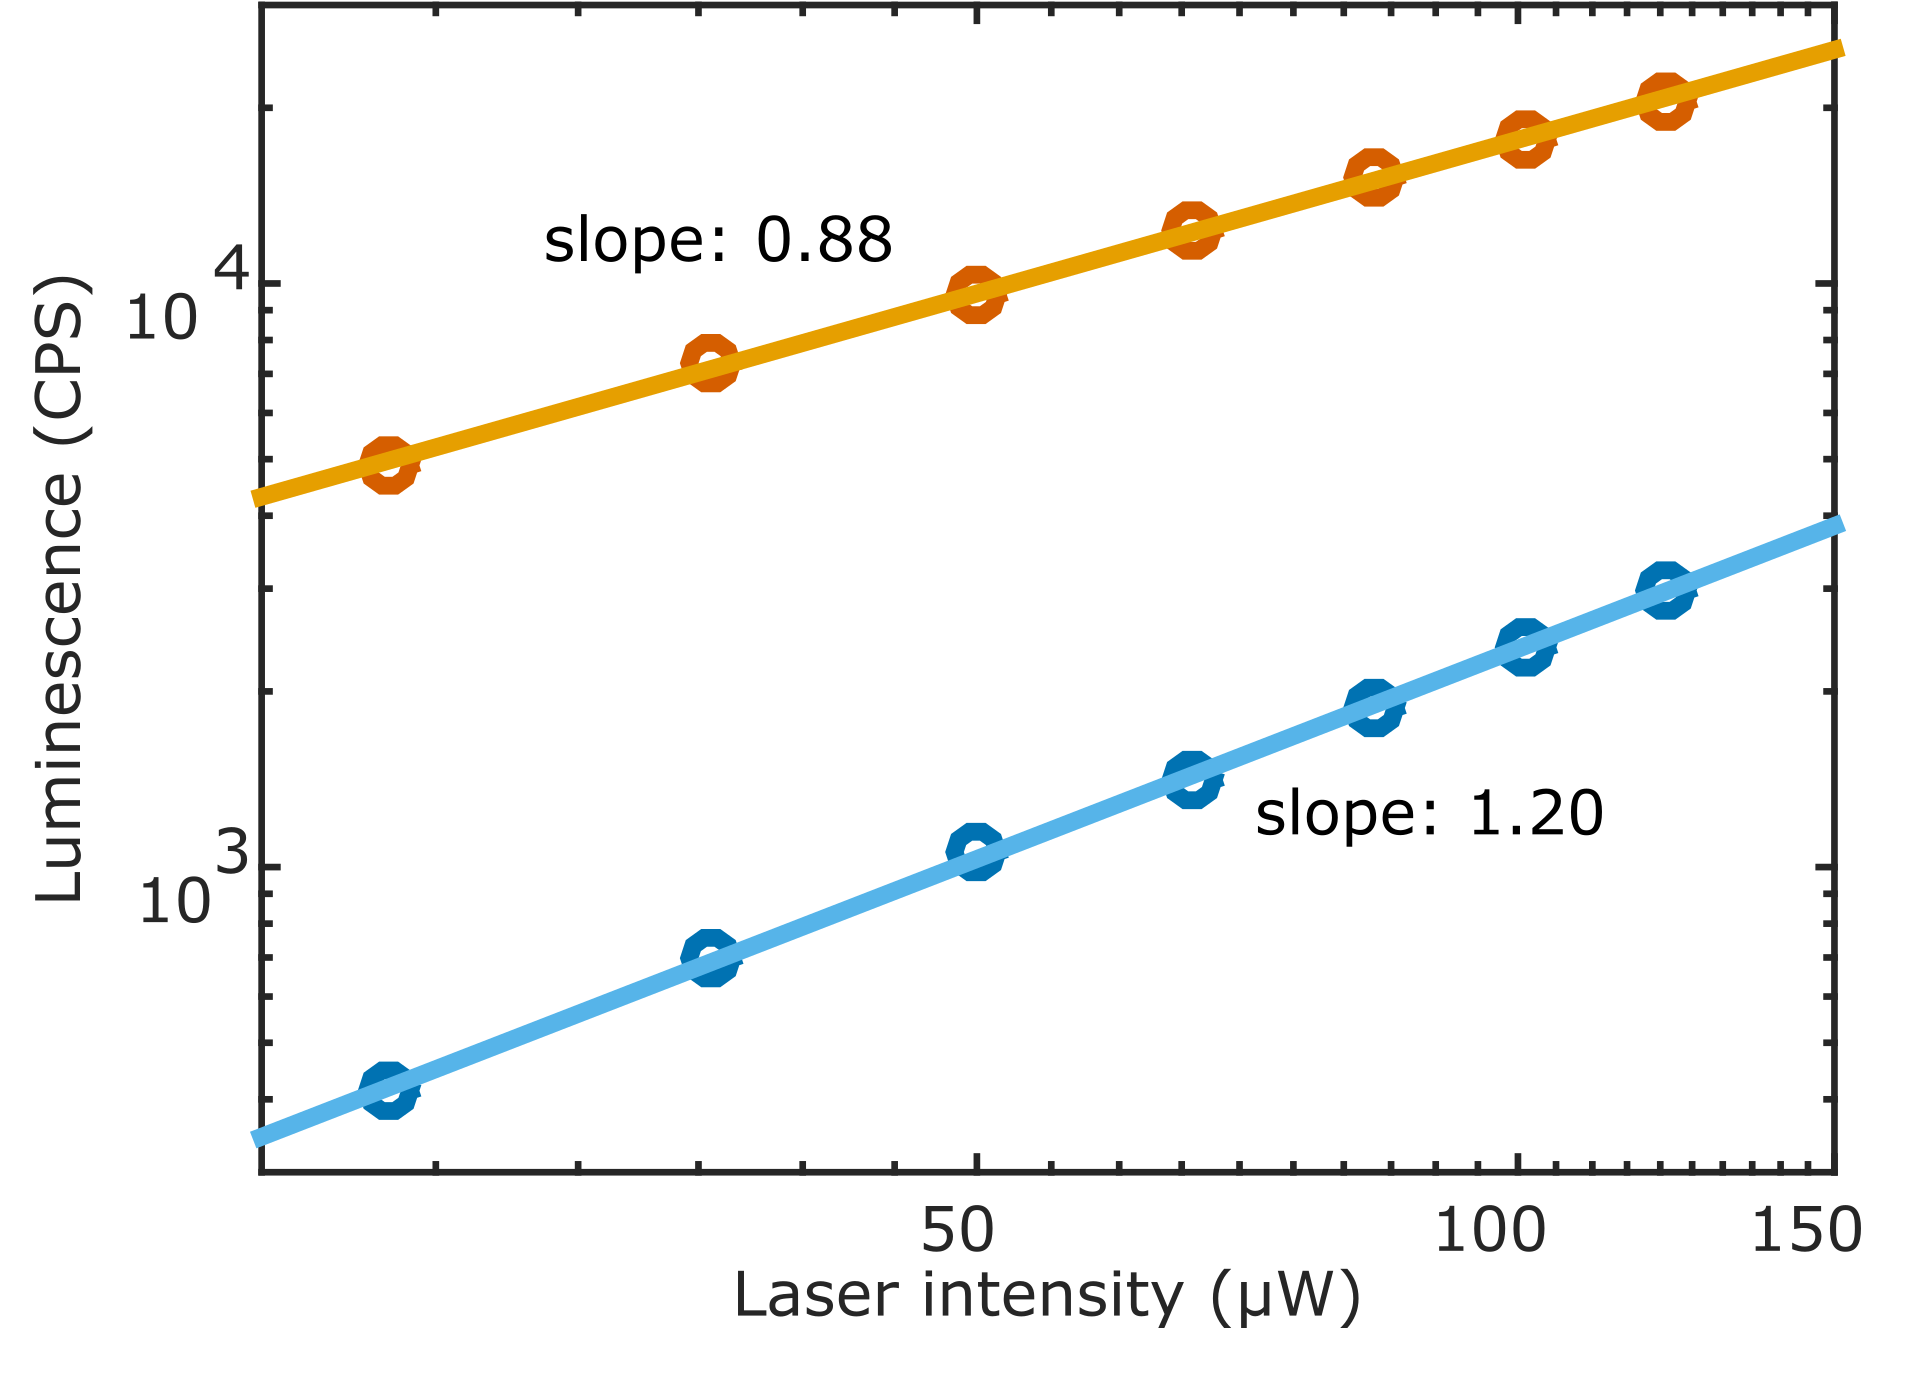
\includegraphics[width=0.45\textwidth]{Chapters/04_Anti-Stokes/Figures/Supplementary/01_AS_S_in_Log/01_AS_S_in_Log.png}
\caption{Stokes and anti-Stokes emission as functions of excitation power. The
linear fit in logarithmic scale has a slope of $0.88$ and $1.20$ respectively,
confirming the 1-photon nature of both kinds of emission.}
	\label{fig:Log_Plot}
\end{figure}

Figure \ref{fig:Log_Plot} shows the power dependence of both the Stokes and
anti-Stokes luminescence. The fit in logarithmic scale ensures that both
processes are due to one photon absorption. 

% \section{Determination of the error in the temperature
% extraction}\label{sec:discussion_errors} Together with the excitation intensity,
% the plasmon position has a crucial role in the accuracy of the extracted temperature. The luminescence spectrum acquired
% with the $532\nm$ laser shows an asymmetric shape, due to a broadband
% contribution from gold added to the plasmonic emission. This makes the initial
% fitting needed for the SPR function of equation \ref{eqn:fitting} non univocally
% determined. For the particle shown in Fig. \ref{fig:spectra_rod}, changing the
% initial wavelength of the fit from $600\nm$ to $640\nm$ yields a significative
% difference in the obtained parameters of the lorentzian.
% 
% \begin{figure}[htp] \centering
% 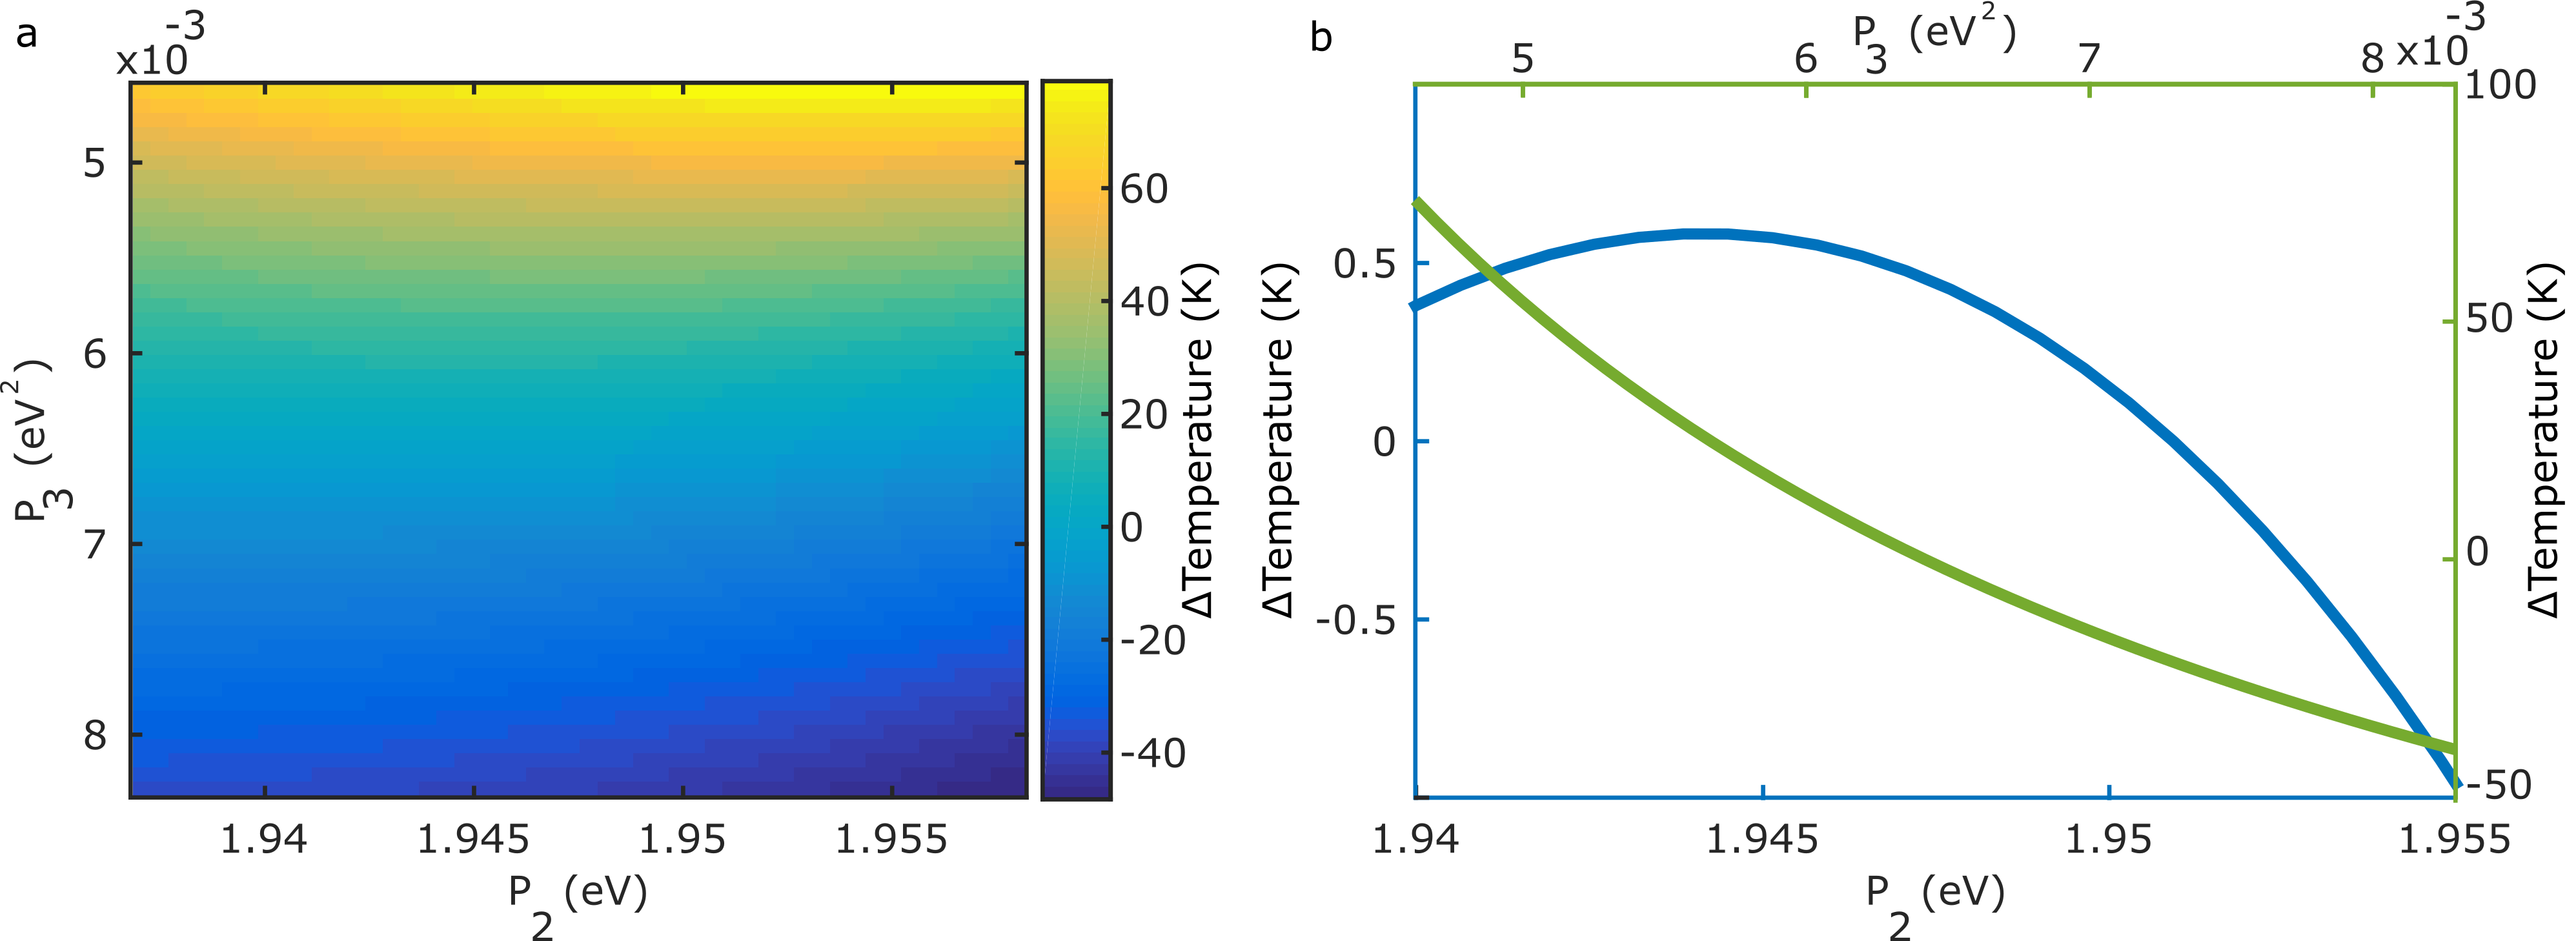
\includegraphics[width=0.90\textwidth]{Chapters/04_Anti-Stokes/Figures/05_Estimation_error/05_estimation_error.png}
% \caption{Estimation of the error due to different fitting parameters of the
% plasmon spectrum. a) 2D grid of the difference in temperature obtained while
% varying both $P_2$ and $P_3$ parameters of the fit. b) Temperature dependence
% while keeping either $P_2$ or $P_3$ constant.}
% 	\label{fig:estimation-error}
% \end{figure}
% 
% Using the following expression for the $I_\textrm{SPR}$ function in $\eV$, 
% \begin{equation*}
% I_\textrm{SPR}(E) = \frac{P_1}{(E-P_2)^2+P_3}
% \end{equation*}
% The different fitting ranges give values for $P_2$ between $1.940\eV$ and
% $1.955eV$, while the values of $P_3$ lie in between $5\cdot10^{-3}\eV^2$ and
% $8\cdot10^{-3}\eV^2$. Figure \ref{fig:estimation-error}.a shows the extracted
% temperature difference from the anti-Stokes spectra for all the possible
% parameter combinations in the range just mentioned. Figure \ref{fig:estimation-error}.b
% shows the temperature dependence while keeping either $P_2$ or $P_3$ constant.
% 
% In this example it is possible to note that the extracted temperature is highly
% dependent on the fitted width of the plasmon spectrum but barely dependent on
% the extracted peak position. From the initial spectrum of the particle, it is
% possible to note that the wing of the plasmon coincides with the range of
% anti-Stokes emission. Therefore minute changes in the initial shape will yield
% higher changes in the extracted temperature.
% 
% This assertion implies that there should be particles in which the extracted
% temperature wouldn't be too sensitive to the initial plasmon fit. To explore
% these possibilities, we calculated the anti-Stokes emission of different
% particles at $400\K$ by using equation \ref{eqn:fitting} and the results of ADDA
% calculations for the SPR function. We then extracted a temperature from these
% spectra while varying the lorentzian parameters as was done for the experimental
% results. In this way it is possible to study the expected error in temperature
% generated by the initial uncertainty in the fitting of the plasmon for different
% particles. 
% 
% \begin{figure}[htp] \centering
% 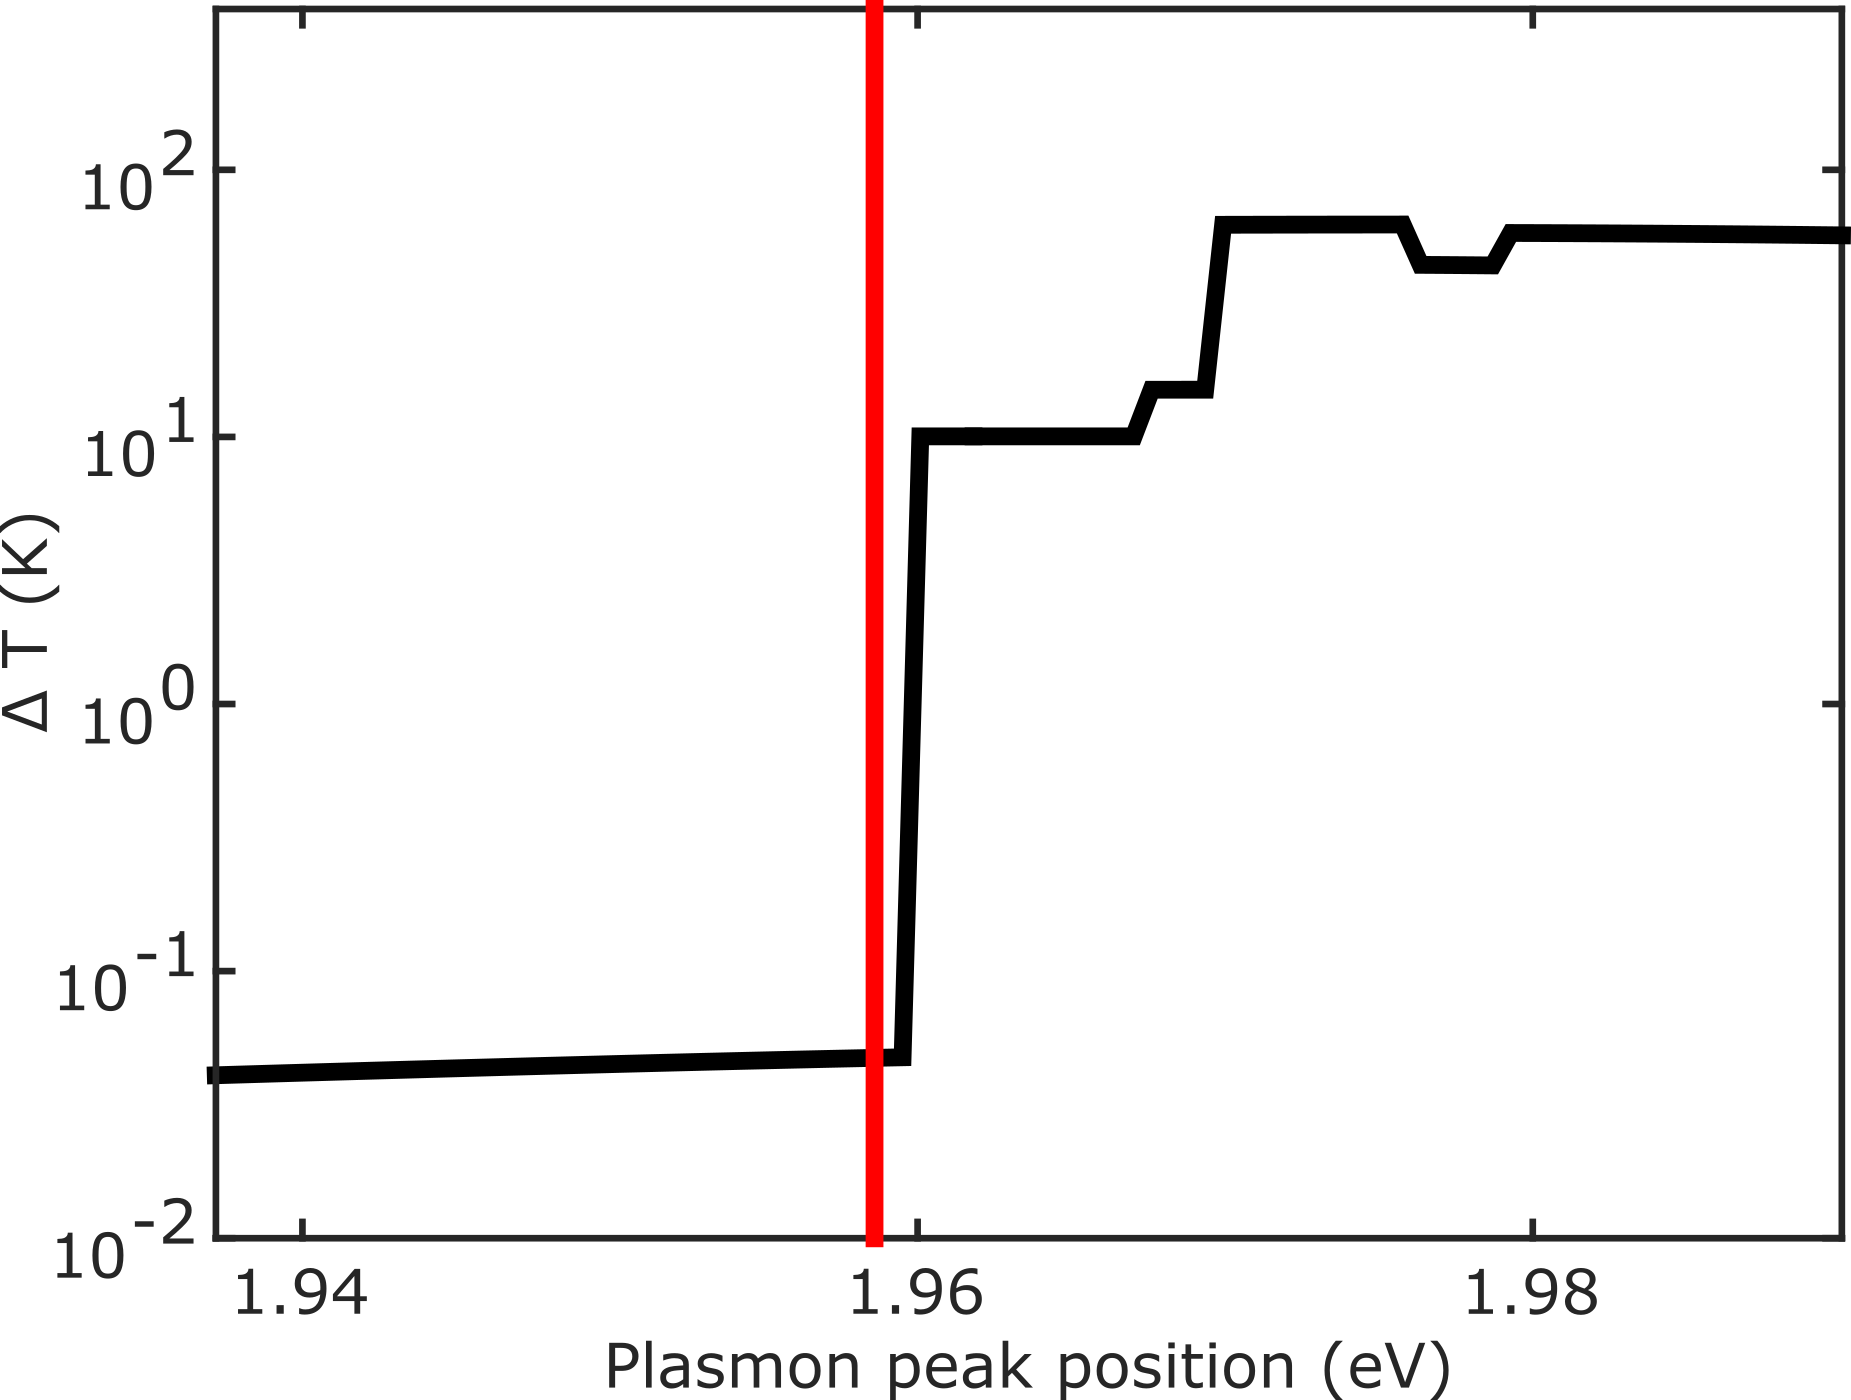
\includegraphics[width=0.45\textwidth]{Chapters/04_Anti-Stokes/Figures/06_Calculation_error/06_calculation_error.png}
% \caption{Calculated error in the temperature extraction due to the uncertainty
% in the plasmon parameters as a function of the resonance position of the
% particle. Clearly, when exciting at the blue wing of the plasmon, the effect of
% these uncertainties is much lower.}
% 	\label{fig:calculated-error}
% \end{figure}
% 
% Figure \ref{fig:calculated-error} shows the uncertainty in the extracted
% temperature as a function of the plasmon peak position. The uncertainty is
% defined as the difference of the maximum and the minimum extracted temperatures
% while varying $P_2$ by $10\%$ and $P_3$ by $30\%$. The vertical red line depicts
% the position of the laser. It is remarkable the difference for particles with a
% resonance red-shifted from the excitation laser to particles blue-shifted.
% Indeed, when the plasmon favors the anti-Stokes emission the correct modelling
% of the resonance is crucial for the extraction of temperatures. On the other
% hand, when the plasmon is red-shifted from the excitation, the induced error in
% the extracted temperature is much lower. The amount of collected light is
% another factor to keep into account. When the resonance is red-shifted
% from the laser, the anti-Stokes emission is much weaker and therefore
% accumulating enough photons in the spectrometer requires longer acquisition
% times.